\documentclass[12pt]{article}

\usepackage{amssymb}
\usepackage{caption}
\usepackage{subcaption}
\usepackage{float}
\usepackage{makecell}
\usepackage{amsmath}
\usepackage{graphicx}
\graphicspath{ {./images/} }
\usepackage[utf8]{inputenc}
\usepackage[russian]{babel}
\usepackage{geometry}
 \geometry{
 a4paper,
 left=20mm,
 right=20mm,
 top=20mm,
 bot=20mm,
 }

\begin{document}

\begin{titlepage}
\begin{center}
    {\small НАЦИОНАЛЬНЫЙ ИССЛЕДОВАТЕЛЬСКИЙ УНИВЕРСИТЕТ ИТМО} \\
    {\small Факультет систем управления и робототехники} \\
    \vspace*{10\baselineskip}
    {\LARGEМоделирование динамических систем} \\
    \ \\
    {\LARGEЛабораторная работа №5} \\
    \ \\
    {\LARGE Системы с задержками} \\
    \ \\
    Вариант 2 \\
    \vspace*{10\baselineskip}
    \hfill {\small Выполнил студент:} \\
    \hfill {\small Кирбаба Д.Д. R3338} \\
    \ \\
    \hfill {\small Преподаватель:} \\
    \hfill {\small Семенов Д.М.} \\
    \mbox{}
    \vfill {\smallг. Санкт-Петербург\\2023}
\end{center}
\end{titlepage}

\section*{Задание 1}
Дана следующая система с задержкой:
\[
    \dot{x}(t) = -sign \ x(t-h), \ t \geq 0, \ h > 0,
\]
где $h = 2$ - постоянная задержка, $x(t) = \varphi(t)$ при $t \in [-h, \ 0]$. \\
\ \\
Используя метод шагов, построить график решения системы при
\[
    \varphi(t) = \begin{cases}
                    -t-1, \ t \in [-2, \ -1), \\
                    -(t+1)^2, \ t \in [-1, 0].
              \end{cases}
\]
Ограничимся решением системы на интервале $[-2, \ 2]$. \\
\begin{equation*}
    \begin{split}
        & t \in [0, \ 2], \ x(0) = \varphi(0) = -1, \ \dot{x}(t) = -sign \ \varphi(t-2) \Rightarrow \\
        & \Rightarrow \begin{cases} \dot{x}(t) = -1, \ \varphi(t-2) > 0, \\ \dot{x}(t) = 1, \ \varphi(t-2) < 0, \\ x(t) = C, \ \varphi(t-2) = 0. \end{cases} \Rightarrow \\
    & \Rightarrow \begin{cases} \dot{x}(t) = -1, \ t \in (0, \ 1], \\ \dot{x}(t) = 1, \ t \in (1, \ 2]. \end{cases} \\
    \end{split}
\end{equation*}

\begin{equation*}
    \begin{split}
        & \dot{x}(t) = -1, \ t \in (0, \ 1], \\
        & \int_{x(0)}^{x(t)} dx = - \int_0^t ds \Rightarrow x(t) = -1 - t \Rightarrow x(1)=-2.
    \end{split}
\end{equation*}

\begin{equation*}
    \begin{split}
        & \dot{x}(t) = 1, \ t \in (1, \ 2], \\
        & \int_{x(1)}^{x(t)} dx = \int_1^t ds \Rightarrow x(t) = t-3 \Rightarrow x(2)=-1.
    \end{split}
\end{equation*}

\begin{equation*}
    \begin{split}
        & t \in (2, 4], \ x(2) = -1, \ \dot{x}(t) = -sign \ \varphi(t-2) \Rightarrow \\
        & \Rightarrow \begin{cases} \dot{x}(t) = -1, \ \varphi(t-2) > 0, \\ \dot{x}(t) = 1, \ \varphi(t-2) < 0, \\ x(t) = C, \ \varphi(t-2) = 0. \end{cases} \Rightarrow \\
        & \Rightarrow \dot{x}(t) = 1, \ t \in (2, \ 4] 
    \end{split}
\end{equation*}

\begin{equation*}
    \begin{split}
        & \dot{x}(t) = 1, \ t \in (2, \ 4], \\
        & \int_{x(2)}^{x(t)} dx = \int_2^t ds \Rightarrow x(t) = t-3 \Rightarrow x(4)=1.
    \end{split}
\end{equation*}
Приведем график решения уравнения:
\begin{figure}[H]
    \centering
    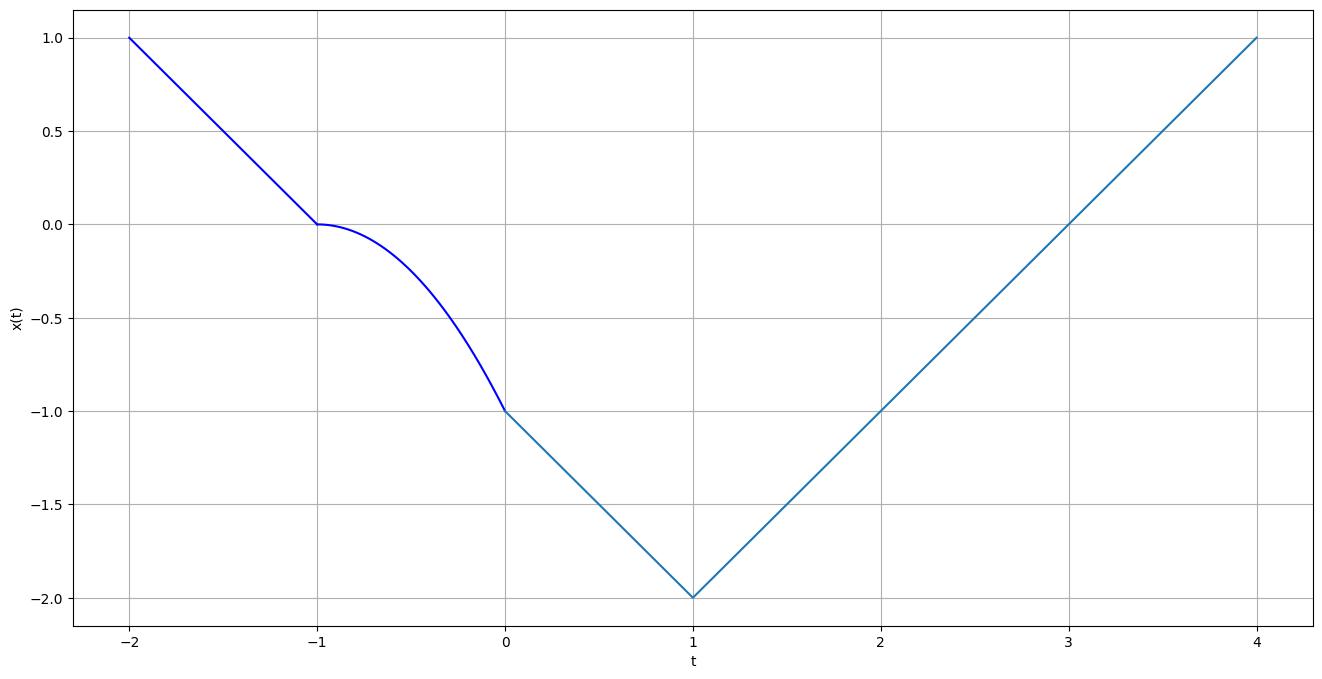
\includegraphics[width=\textwidth]{1_task_plot.png}
    \caption{Решение уравнения при $h = 2$ методом шагов.}
    \label{fig:1_task_plot}
\end{figure}

\section*{Задание 2}
Дана система с некоторой произвольной задержкой $\tau(t)$:
\[
    \dot{x}(t) = -x(t)+0.1x(t-\tau(t))
\]
Построить функцию Ляпунова. С помощью метода Разумихина доказать устойчивость данной системы. Для решения матричных неравенств использовать критерий Сильвестра. \ 
\ \\
Согласно методу Разумихина, система является асимптотически устойчивой, когда разрешимо линейное матричное неравенство $(LMI)$:
\[
    \Psi = \begin{bmatrix}
        A^TP + PA + qP & PA_1 \\
        A_1^TP & -qP
    \end{bmatrix} < 0, \ q>0, \ P>0.
\]
Из уравнения следует, что $A=-1, \ A_1=0.1$. Тогда имеем:
\[
    \Psi = \begin{bmatrix}
        -2P+qP & 0.1P \\
        0.1P & -qP
    \end{bmatrix} < 0, \ q>0, \ P>0.
\]
Неравенство выполнено тогда, когда (критерий Сильвестра):
\[
    \begin{cases}
        -P(2-q) < 0, \\
        qP^2(2-q)-0.01P^2 < 0, \\
        q>0, \ P>0.
    \end{cases}
\]
Из первого неравенства получаем $0 < q < 2$, а из второго неравенства получаем $0.002 < q < 1.998$. Таким образом, система $LMI$ разрешима $\forall q \in (0.002, 1.998) \ \Rightarrow$ система асимптотически устойчива.

\section*{Задание 3}
Дана система с постоянной задержкой $h$:
\[
    \dot{x}(t) = Ax(t)+A_1x(t-h),
\]
где $A = \begin{bmatrix}
    -3 & -1 \\
    1 & -3
\end{bmatrix}, \ A_1 = \begin{bmatrix}
    -2 & 1 \\
    0 & -1
\end{bmatrix}, \ h = 2, \ x \in \mathbb{R}$.\\
\ \\

\begin{figure}[H]
    \centering
    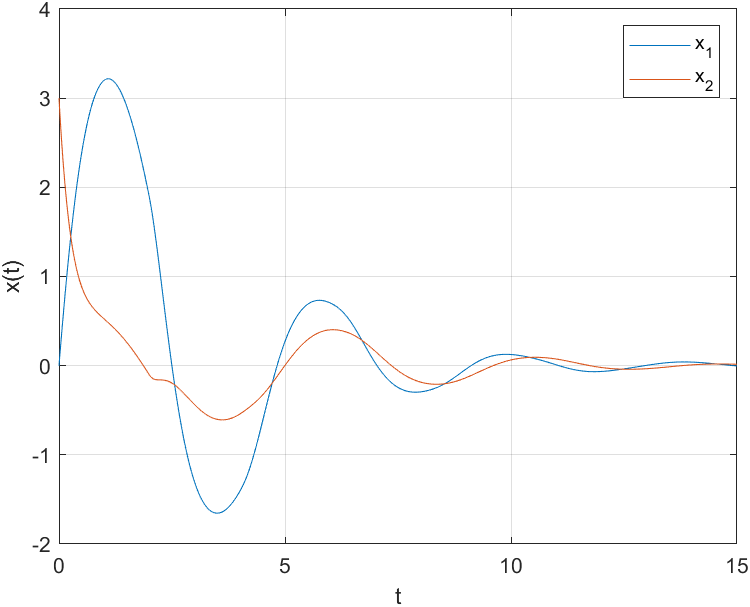
\includegraphics[width=0.7\textwidth]{3_task_modeling.png}
    \caption{Моделирование системы с задержкой $h=2$.}
    \label{fig:3_task_modeling}
\end{figure}

Для доказательства устойчивости с помощью функционала Ляпунова-Красовского необходимо решить матричное уравнение вида:
\[
    \Psi = \begin{bmatrix}
        A^TP + PA + Q & A_1P \\
        A_1^TP & -Q
    \end{bmatrix} < 0, \ Q > 0, \ P > 0.
\]
так как задержка постоянная, то $\dot{h} = 0$. Решения данного $LMI$ в MATLAB дает следующий результат:

\[
    P = \begin{bmatrix}
        7.9318 & 0.5348 \\
        0.5348 & 10.0707
    \end{bmatrix}, \ Q = \begin{bmatrix}
        25.6439 & 0.3566 \\
        0.3566 & 30.6347
    \end{bmatrix}
\]
Следовательно, данная система является устойчивой.

\section*{Выводы}
В данной работе были исследованы системы с задержками. \\
В первой части работы был применен метод шагов для решения системы. Также был построен график переходного процесса. \\
Во второй части было проведено исследование систем с запаздыванием на устойчивость. В качестве анализа было реализовано два метода: Ляпунова-Красовского и Разумихина. Результаты работы удовлетворительно, предпложенные системы были устойчивы. Также, при применении метода Ляпунова-Красовского матричный неравенства решались с помощью библиотеки YALMIP для MATLAB.

\end{document}